% Dissertation-ready template: Method of Manufactured Solutions (MMS)
% This file intentionally contains no report prose. Replace bracketed prompts
% and comment blocks with evidence drawn from the stored result directories.
\documentclass[11pt,a4paper]{article}

\usepackage[margin=28mm]{geometry}
\usepackage{amsmath,amssymb,bm}
\usepackage{booktabs,threeparttable}
\usepackage{graphicx}
\usepackage{siunitx}
\usepackage{hyperref}
\usepackage{cleveref}
\usepackage{xcolor}
\usepackage{makecell}
\usepackage[backend=biber, style=numeric]{biblatex}
\addbibresource{references.bib}


\graphicspath{{../}{solns/mms_adaptive_temperature_error/}}
\newcommand{\placeholderfigure}[2]{%
  \fbox{\parbox[c][#2][c]{0.92\linewidth}{\centering\textit{Figure placeholder}\\[0.5em]#1}}%
}
\newcommand{\norm}[1]{\left\lVert #1 \right\rVert}
\newcommand{\seminorm}[1]{\left\lvert #1 \right\rvert}

\title{Verification of a Two-Dimensional Conjugate Heat-Transfer Solver\\
       by the Method of Manufactured Solutions}
\author{Branislav Palúch}
\date{\today}

\begin{document}
\maketitle

\begin{abstract}
% 150--220 words. State the verification objective, equations verified,
% discretisation range, the principal flow result, temperature-verification
% status, and one precise limitation. Do not explain the entire methodology.
abstract's waiting for the report to be finished
\end{abstract}

\section{Introduction and verification scope}
% Target: 0.5--1 page.
% Explain why code verification is needed before interpreting physical CHT
% simulations. Define MMS as verification of the implemented equations and
% discretisation, not validation against experiment. State the scope exactly:
% 2D, steady, unit-square, smooth solution, global refinement, fluid domain.
% Explicitly exclude unverified claims: physical-model validity, transient
% behaviour, 3D, and fluid--solid MMS unless supporting results are added.
Code verification is an important step towards successfull simulation.
It concerns whether our code correctly implements mathematical model of studied phenomenon \cite{roy2005verification}.
It does not however judge how well the chosen model describes reality.

Method of Manufactured Solution (MMS) is a general code verification tool \cite{salari2000mms}.
Workflow of MMS is following:
\begin{enumerate}
  \item Choose an appropriate analytical field.
  \item Compute corresponding boundary conditions.
  \item Substitute the field into governing equations and get source terms.
  \item Solve numerically with computed source terms and boundary conditions.
  \item Compute cell errors and combine them into a global error using appropriate norm.
  \item Repeat for gradually refined grid and compare the error convergence with theoretical values.
\end{enumerate}


MMS is used here to verify implementation of conjugate heat tranfer solver.
The problem is in 2D and we are considering a steady-state.
The domain is a fluid-only unit square.
The square mesh is refined globally each time for easier convergence analysis.




\section{Mathematical model and discretisation}
% Target: 1--1.5 pages. Use the notation actually used by the solver.
\subsection{Governing equations}
% Give the steady incompressible Navier--Stokes equations and the steady
% advection--diffusion temperature equation. Define u, p, T, nu, kappa, f, s.

The mathematical model that is implemented in the code is described by following equations:

\begin{subequations}\label{cht}
  \begin{align}
    (\bm{u}\cdot\nabla)\bm{u}-\nu\Delta\bm{u}+\nabla p &= \bm{f}, \label{cht-momentum}\\
    \nabla\cdot\bm{u} &= 0, \label{cht-continuity} \\
    \bm{u}\cdot\nabla T-\kappa\Delta T &= s, \label{cht-heat}
  \end{align}
\end{subequations}  


where $\bm{u}$ is fluid velocity field, $\nu$ is viscosity, $p$ is pressure, $\bm{f}$ is external force (source term), $T$ is temperature, $\kappa$ is thermal diffusivity and $s$ is a heat source.
The \eqref{cht-momentum} and \eqref{cht-continuity} are incompressible Navier-Stokes equations, top one governing momentum of fluid and the other one ensuring its incompressibility (also called continuity equation).
The advection-diffusion temperature equation \ref{cht-heat} concerns heat transport by conduction and motion of the fluid.  



\subsection{Finite-element approximation and error norms}
% State the Taylor--Hood pair precisely. In the present code, ``degree k''
% corresponds to Q_{k+1}/Q_k for velocity/pressure; verify and state the
% temperature polynomial space from the implementation before finalising.
% Define L2(u), L2(p), H1(u), and L2(T). Mention global mesh refinement,
% five refinement levels, and the pressure mean-value adjustment.
% Give expected asymptotic rates only after checking the exact FE spaces.
The code aims to implement a finite-element approximation of of the model above.
Taylor-Hood elements are used, i.e. polynomial basis functions used for discretizing velocity are one degree higher than those for pressure.
This element pair satisfies the inf-sup stability condition which ensures a robust discretization \cite{taylor1973numerical,brezzi1991stability}.
Degree for temperature elements was set same to degree of velocity elements.
Simulation with degree $k$ basis functions thus should be understand as pressure being approximated with $k$ degree polynomials and velocity with temperature with $k+1$ degree polynomials.

Quality of the numerical solution is measured via an error $e$ defined as the difference between computed and manufactured analytical solution on a relevant domain $\Omega$.
For measuring the difference, we use $L^2$ norm and $H^1$ seminorm:
\begin{subequations}
  \begin{align}
    e_{u, L^2(\Omega)} &= \left\|u_h - u_{\mathrm{MMS}}\right\|_{L^2(\Omega)} =
    \left(
      \int_{\Omega}
      \left|u_h - u_{\mathrm{MMS}}\right|^2
      \,\mathrm{d}x
    \right)^{1/2}, \\
    e_{u,H^1(\Omega)}
      &= \left|u_h-u_{\mathrm{MMS}}\right|_{H^1(\Omega)} =
      \left(
      \int_{\Omega}
      \left|\nabla u\right|^2
      \,\mathrm{d}x
      \right)^{1/2} ,
  \end{align}
\end{subequations}
where $u$ is concerned quantity (vector/scalar), in particular $u_h$ is discretized solution and $u_{MMS}$ is manufactured analytical solution.
We use $L^2$ norm for error on velocity, pressure and temperature and $H^1$ norm for velocity.

\section{Manufactured problem}
% Target: 1.5--2 pages. The exact expressions and source terms are generated
% from scripts/expressions_mms.py. Regenerate mms_report.tex if expressions
% change; include the generated equations rather than retyping them manually.
The manufactured solution ground truth is given by \texttt{scripts/expressions\_mms.py}.
From this source the exact solution, forcing terms and boundary conditions for C++ solver are generated.
Also LaTex expressions stated here are generated based on this file.


\subsection{Exact fields, forcing, and boundary data}
% \section*{Manufactured solution}
This report defines a steady MMS pair on $\Omega=[0,1]\times[0,1]$.

\subsection*{Exact fields}
\[u_x(x,y) = \sin{\left(\pi x \right)} \cos{\left(\pi y \right)}\]
\[u_y(x,y) = - \sin{\left(\pi y \right)} \cos{\left(\pi x \right)}\]
\[p(x,y) = \sin{\left(\pi y \right)} \cos{\left(\pi x \right)}\]
\[T(x,y) = \sin{\left(\pi y \right)} \cos{\left(2 \pi x \right)}\]

\subsection*{Governing equations}
For momentum we assume the steady incompressible Navier--Stokes residual
$ (u \cdot \nabla)u - \nu \Delta u + \nabla p - f = 0$, with $\nabla \cdot u = 0$.
For temperature we assume steady advection--diffusion
$u \cdot \nabla T - \kappa \Delta T - s = 0$.

\subsection*{Source terms}
\[f_x(x,y) = \pi \left(2 \pi \nu \cos{\left(\pi y \right)} - \sin{\left(\pi y \right)} + \cos{\left(\pi x \right)}\right) \sin{\left(\pi x \right)}\]
\[f_y(x,y) = \frac{\pi \left(2 \pi \nu \sin{\left(\pi \left(x - y\right) \right)} - 2 \pi \nu \sin{\left(\pi \left(x + y\right) \right)} + \sin{\left(2 \pi y \right)} + \cos{\left(\pi \left(x - y\right) \right)} + \cos{\left(\pi \left(x + y\right) \right)}\right)}{2}\]
\[\nabla \cdot u = 0\]
\[s(x,y) = \frac{\pi \left(- 20 \pi \kappa \sin^{2}{\left(\pi x \right)} + 10 \pi \kappa - 3 \cos{\left(\pi x \right)} \cos{\left(\pi y \right)} + \cos{\left(3 \pi x \right)} \cos{\left(\pi y \right)}\right) \sin{\left(\pi y \right)}}{2}\]

\subsection*{Boundary values on $\partial\Omega$}
\paragraph*{$u_x$}
\[x = 0: 0\]
\[x = 1: 0\]
\[y = 0: \sin{\left(\pi x \right)}\]
\[y = 1: - \sin{\left(\pi x \right)}\]
\paragraph*{$u_y$}
\[x = 0: - \sin{\left(\pi y \right)}\]
\[x = 1: \sin{\left(\pi y \right)}\]
\[y = 0: 0\]
\[y = 1: 0\]
\paragraph*{$p$}
\[x = 0: \sin{\left(\pi y \right)}\]
\[x = 1: - \sin{\left(\pi y \right)}\]
\[y = 0: 0\]
\[y = 1: 0\]
\paragraph*{$T$}
\[x = 0: \sin{\left(\pi y \right)}\]
\[x = 1: \sin{\left(\pi y \right)}\]
\[y = 0: 0\]
\[y = 1: 0\]
% Insert the complete generated momentum and temperature source terms here,
% or move their long forms to an appendix and cite it. State that the velocity
% is divergence-free and that Dirichlet data are exact traces of these fields.
According to \href{https://dealii.org/current/doxygen/deal.II/step_7.html#step_7-Themethodofmanufacturedsolutions}{Deal II tutorial 7}, the chosen solution should have certain characteristics.
\begin{enumerate}
  \item not too complicated
  \item not a polynomial of low degree - to avoid superconvergence
  \item sufficiently smooth - theoretical FEM convergence estimates typically assume this
  \item with characteristic lenght bigger than a mesh cell - to be able to approximate it reasonably.
\end{enumerate}
We chose following solution consisting of goniometric functions that satisfies these criterions:
\begin{subequations}
  \begin{align}
    u_x(x,y) &= \sin{\left(\pi x \right)} \cos{\left(\pi y \right)} \\
    u_y(x,y) &= - \sin{\left(\pi y \right)} \cos{\left(\pi x \right)} \\
    p(x,y) &= \sin{\left(\pi y \right)} \cos{\left(\pi x \right)} \\
    T(x,y) &= \sin{\left(\pi y \right)} \cos{\left(2 \pi x \right)}.
  \end{align}
\end{subequations}
Also the velocity is designed to be divergence-free to satisfy the continuity equation.
The solution is visualized on figure \ref{fig:mms-fields} together with computed source fields whose analytical forms can be found in appendix \ref{appendix:generated_sources}.
The boundaray conditions are implemented as functions by sampling from the analytical solution, thus the analytical terms are unnecessary to state here.

\begin{figure}[htbp]
  \centering
  % Replace this placeholder with:
  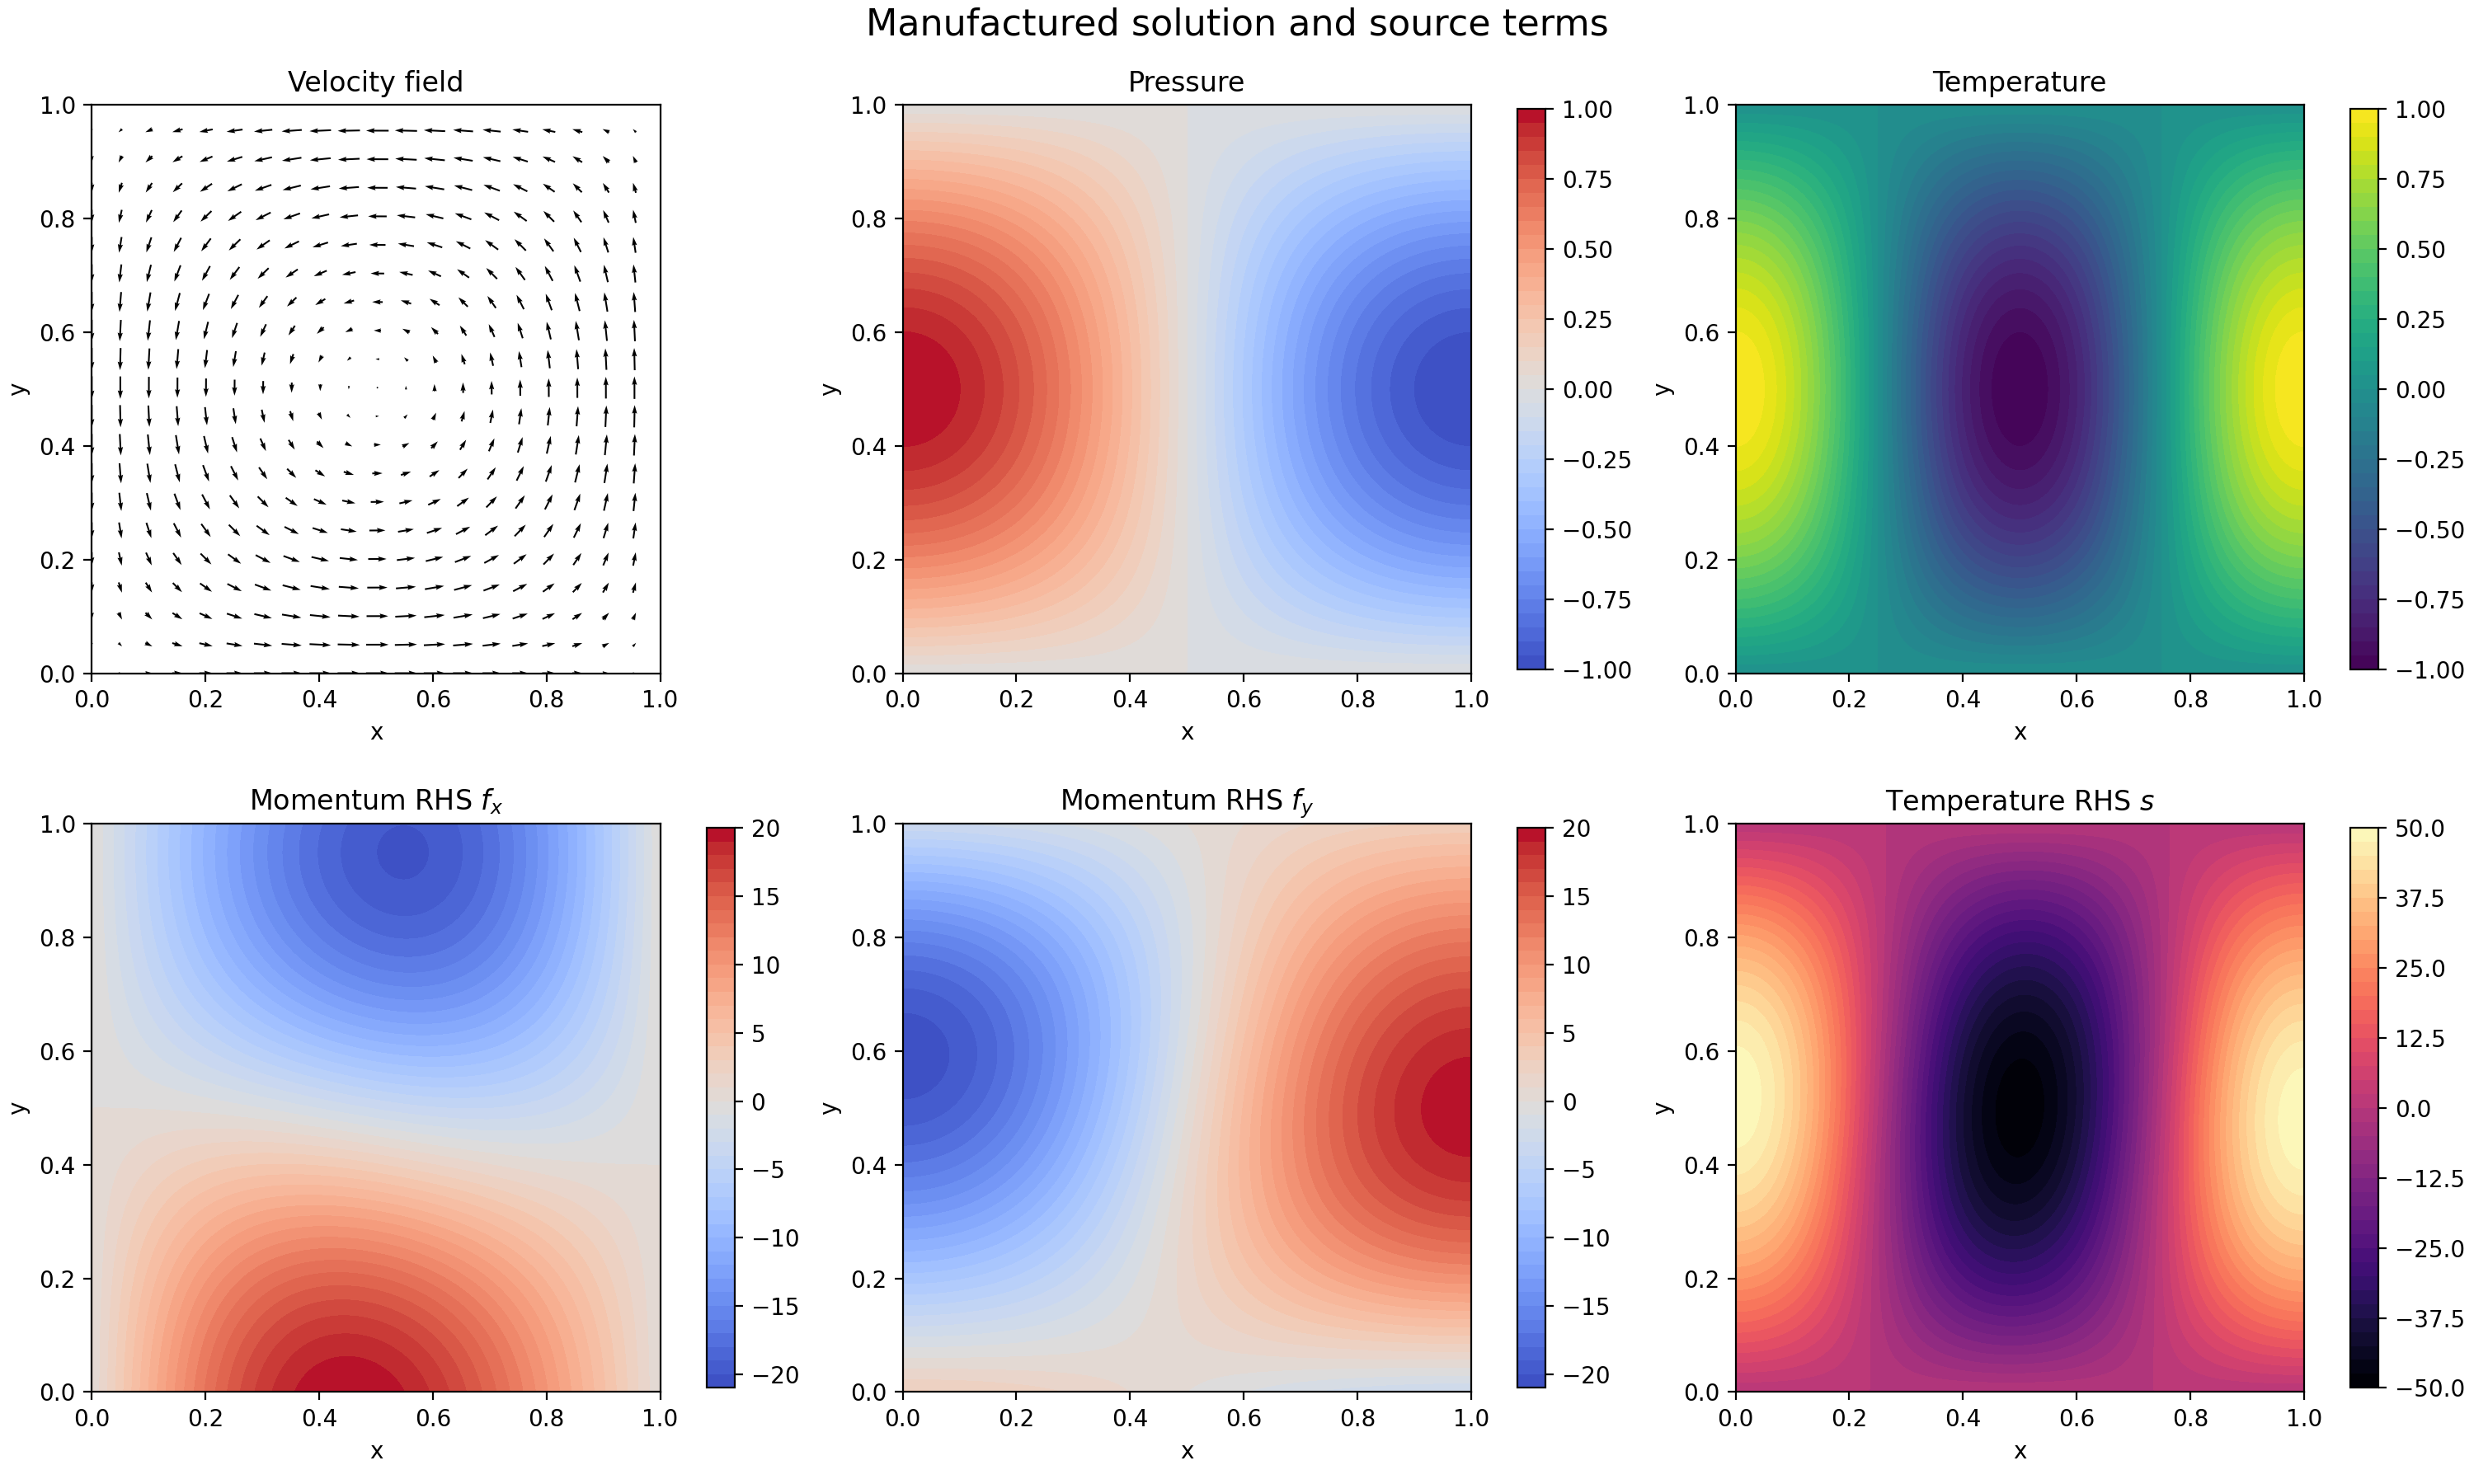
\includegraphics[width=\linewidth]{mms_visualization.png}
  \caption{visualization of the manufactured solution and computed forcing terms.}
  \label{fig:mms-fields}
\end{figure}


\section{Computational verification procedure}
% Target: 1--1.5 pages.
% Report: square and square_finer meshes, Re=100 and Re=7500, degrees 1--3,
% number of refinement cycles, thermal diffusivity, nonlinear stopping rule,
% quadrature order, and how the fitted slopes are obtained. Include a short
% reproducibility paragraph: case files, output directory convention, and
% the script used for fitting. Do not report a fit that contains a numerical
% error floor without identifying/excluding those points.
The verification was made on a square grid with initial number of cells per side 17.
The grid was four times globally refined and error at each refinement was recorded.
The number of cells and degrees of freedom for each refinement are stated in table \ref{tab:refinements}.
Verification was made for two Reynolds numbers (100 and 7500) and for three degrees of basis functions ($Q_2/Q_1, Q_3/Q_2$ and $Q_4/Q_3$).
BOOKMARK

\begin{table}[htbp]
  \centering
  \caption{Verification matrix and data availability.}
  \label{tab:refinements}
  \begin{tabular}{ccc}
    \toprule
    cycle & \# cells & \# dofs\\ 
    \midrule
    0 & 289 & 12226 \\
    1 & 1156 & 48147 \\
    2 & 4624 & 191083 \\
    3 & 18496 & 761331 \\
    4 & 73984 & 3039331 \\
    \bottomrule
  \end{tabular}
\end{table}


\section{Flow verification results}
% Target: 3--4 pages. This is the principal completed result.
% First give expected rates, then measured rates with standard errors. Discuss
% Re=100 and Re=7500 separately. Do not claim agreement merely because a
% rounded value is close: discuss uncertainty, local rates, and asymptotic
% range. Explicitly discuss the degree-1 H1 result at Re=7500.


\begin{figure}[htbp]
  \centering
  % Suggested source figures: error-global-q*_L2_velocity.png,
  % error-global-q*_L2_pressure.png, error-global-q*_H1_velocity.png.
  % Prefer a clean 1x3 composite for one degree or one 3x3 composite across
  % degrees; use consistent axes and identify Re in the caption.
  \placeholderfigure{Log--log flow-error convergence plots.}{65mm}
  \caption{[Caption: norms, Reynolds number, polynomial degrees, fit range,
  and whether all refinement levels are included.]}
  \label{fig:flow-convergence}
\end{figure}

\section{Coupled temperature verification}
% Target: 1.5--2 pages. Describe the added thermal source term, MMS thermal
% Dirichlet conditions, temperature error integration, and solver tolerance.
% At Re=100 there are results for degrees 1--3. Degree 1 gives a stable rate;
% degree 2 and 3 temperature errors become floor-dominated on fine meshes.
% Therefore report raw errors and local rates, but fit only defensible points
% or label full-range fits as non-asymptotic diagnostics. There are presently
% no corresponding coupled temperature runs at Re=7500.


  % Requires \usepackage{xcolor,makecell}
\begin{table}[htbp]
\centering
\begin{tabular}{|r|r|r|r|r|r|r|r|r|}
\hline
cycle & \makecell{$L^{2}$\\velocity} & rate & \makecell{$L^{2}$\\pressure} & rate & \makecell{$H^{2}$\\velocity} & rate & \makecell{$L^{2}$\\temper.} & rate \\ \hline
0 & 4.634e-09 & \makecell{--} & 1.640e-07 & \makecell{--} & 9.531e-07 & \makecell{--} & 4.305e-08 & \makecell{--} \\ \hline
1 & 1.037e-10 & 5.48 & 1.023e-08 & 4.00 & 4.949e-08 & 4.27 & 1.347e-09 & 5.00 \\ \hline
2 & 2.804e-12 & 5.21 & 6.416e-10 & 4.00 & 2.907e-09 & 4.09 & 4.212e-11 & 5.00 \\ \hline
3 & 8.987e-14 & 4.96 & 4.001e-11 & 4.00 & 1.786e-10 & 4.03 & \textcolor{red}{2.985e-12} & \textcolor{red}{3.82} \\ \hline
4 & \textcolor{red}{6.668e-14} & \textcolor{red}{0.43} & 2.500e-12 & 4.00 & 1.113e-11 & 4.00 & \textcolor{red}{5.880e-12} & \textcolor{red}{-0.98} \\ \hline
\makecell[r]{fitted\\rate} & \makecell{--} & \makecell[r]{$5.22 $\\$\pm  0.08$} & \makecell{--} & \makecell[r]{$4.0003 $\\$\pm  0.0006$} & \makecell{--} & \makecell[r]{$4.09 $\\$\pm  0.03$} & \makecell{--} & \makecell[r]{$4.99866 $\\$\pm  0.00019$} \\ \hline
expect & \makecell{--} & $5$ & \makecell{--} & $4$ & \makecell{--} & $4$ & \makecell{--} & $5$ \\ \hline
\end{tabular}
\caption{Local convergence rates computed from adjacent refinement levels. Pressure is approximated with degree-$3$ polynomials, while velocity and temperature are approximated with degree-$4$ polynomials. Red values are fine-grid outliers excluded from the log-log least-squares fit. The final two rows show fitted and theoretical rates, respectively.}
\end{table}


\begin{figure}[htbp]
  \centering
  % Suggested source figures: error-global-q*_L2_temperature.png from the
  % *_temperature_tighter directories. Make one composite plot if needed.
  \placeholderfigure{Temperature convergence plot, with floor-dominated
  refinement levels visibly distinguished.}{58mm}
  \caption{[Caption: state the fit range and explain any excluded points.]}
  \label{fig:temperature-convergence}
\end{figure}

\section{Spatial error diagnostics}
% Target: 0.75--1.5 pages. Explain that per-cell integrated errors diagnose
% spatial localisation and implementation problems; they are not a replacement
% for global convergence rates. Discuss only patterns visible in the figure.
% Use the final, consistent data set and specify Re, degree, and refinement.

\begin{figure}[htbp]
  \centering
  % Start from mms_integral_errors.png, but crop/rebuild a publication-sized
  % subset rather than inserting its entire dense 3x4 layout.
  \placeholderfigure{Selected per-cell velocity L2, velocity H1, and pressure
  L2 error fields.}{62mm}
  \caption{[Caption: identify the result set and explain colour-bar scaling.]}
  \label{fig:cell-errors}
\end{figure}

\section{Limitations and remaining verification work}
% Target: 0.75--1 page. Be explicit and constructive.
% Required: (i) thermal convergence at Re=7500 is missing; (ii) degree-2/3
% thermal fine-mesh results need a floor-aware analysis or reruns with a
% demonstrated tolerance criterion; (iii) the MMS is 2D/smooth/fluid-only;
% (iv) a separate manufactured fluid--solid problem would be required to claim
% verification of conjugate interface coupling.

\section{Conclusions}
% Target: 0.4--0.7 page. Give 3--5 numbered conclusions answering: what has
% been implemented, which flow claims are supported, what is supported for
% temperature, and the next experiment needed to close the verification matrix.

\appendix
\section{Generated MMS forcing terms and boundary values}\label{appendix:generated_sources}
% Paste or \input the generated mms_report.tex material here after checking
% it matches the code version used to produce the reported results.
\begin{subequations}
  \begin{align}
    f_x(x,y) &= \pi \left(2 \pi \nu \cos{\left(\pi y \right)} - \sin{\left(\pi y \right)} + \cos{\left(\pi x \right)}\right) \sin{\left(\pi x \right)} \\
    f_y(x,y) &= \frac{\pi}{2} \left(2 \pi \nu \sin{\left(\pi \left(x - y\right) \right)} - 2 \pi \nu \sin{\left(\pi \left(x + y\right) \right)} \right. \\ \notag
    & \left. + \sin{\left(2 \pi y \right)} + \cos{\left(\pi \left(x - y\right) \right)} + \cos{\left(\pi \left(x + y\right) \right)}\right) \\
    s(x,y) &= \frac{\pi}{2} \left(- 20 \pi \kappa \sin^{2}{\left(\pi x \right)} + 10 \pi \kappa - 3 \cos{\left(\pi x \right)} \cos{\left(\pi y \right)} \right. \\ \notag
    &+ \left. \cos{\left(3 \pi x \right)} \cos{\left(\pi y \right)}\right) \sin{\left(\pi y \right)}
  \end{align}
\end{subequations}

\section{Complete convergence tables}
% Include the generated convergence_rates.tex tables for every reported set.
% Put exploratory/obsolete directories in a separate archival appendix or omit
% them. Record the exact result-directory names for reproducibility.

\printbibliography

\end{document}
